
% bp                  Physical pain in the last 4 weeks
% gh                  Current general health
% pf1                 State of health affects ascending stairs
% pf2                 State of health affects tiring tasks
% rp1                 Accomplished less due to physical problems
% rp2                 Limitations due to physical problems
% mh1                 Run-down, melancholy in the last 4 weeks
% mh2                 Well-balanced in the last 4 weeks
% vt                  Physical pain in the last 4 weeks
% re1                 Accomplished less due to emotional problems
% re2                 Less careful due to emotional problems
% sf                  Limited socially due to health



\begin{figure}[ht!]
  A: Physical Health
  \\  %%%%%%%%%%%%%%%%%%%%%%%%%%%%%%%%%%%%%%%%%%%%%%%%%%%%%%%%%%%%%% newline 
  \begin{subfigure}{.30\textwidth}
    \includegraphics[width=1\linewidth]{descriptives/fig_phys_bp.pdf}
    \caption{\code{bp}: Physical pain in the last 4 weeks}
    \label{fig:bp}
\end{subfigure}\hfill%
  \begin{subfigure}{.30\textwidth}
    \includegraphics[width=1\linewidth]{descriptives/fig_phys_gh.pdf}
    \caption{\code{gh}: Current general health \phantom{text to break line}}
    \label{fig:gh}
\end{subfigure}\hfill%
  \begin{subfigure}{.30\textwidth}
    \includegraphics[width=1\linewidth]{descriptives/fig_phys_pf1.pdf}
    \caption{\code{pf1}: State of health affects ascending stairs}
    \label{fig:pf1}
\end{subfigure}\hfill%
  \\  %%%%%%%%%%%%%%%%%%%%%%%%%%%%%%%%%%%%%%%%%%%%%%%%%%%%%%%%%%%%%% newline 
  \begin{subfigure}{.30\textwidth}
    \includegraphics[width=1\linewidth]{descriptives/fig_phys_pf2.pdf}
    \caption{\code{pf2}: State of health affects tiring tasks}
    \label{fig:pf2}
  \end{subfigure}\hfill%
  \begin{subfigure}{.30\textwidth}
    \includegraphics[width=1\linewidth]{descriptives/fig_phys_rp1.pdf}
    \caption{\code{rp1}: Accomplished less due to physical problems}
    \label{fig:rp1}
  \end{subfigure}\hfill%
  \begin{subfigure}{.30\textwidth}
    \includegraphics[width=1\linewidth]{descriptives/fig_phys_rp2.pdf}
    \caption{\code{rp2}: Limitations due to physical problems}
    \label{fig:rp2}
  \end{subfigure}\hfill%
  \\  %%%%%%%%%%%%%%%%%%%%%%%%%%%%%%%%%%%%%%%%%%%%%%%%%%%%%%%%%%%%%% newline 
  B: Mental Health
  \\  %%%%%%%%%%%%%%%%%%%%%%%%%%%%%%%%%%%%%%%%%%%%%%%%%%%%%%%%%%%%%% newline 
  \begin{subfigure}{.30\textwidth}
    \includegraphics[width=1\linewidth]{descriptives/fig_ment_mh1.pdf}
    \caption{\code{mh1}: Run-down, melancholy in the last 4 weeks}
    \label{fig:mh1}
\end{subfigure}\hfill%
  \begin{subfigure}{.30\textwidth}
    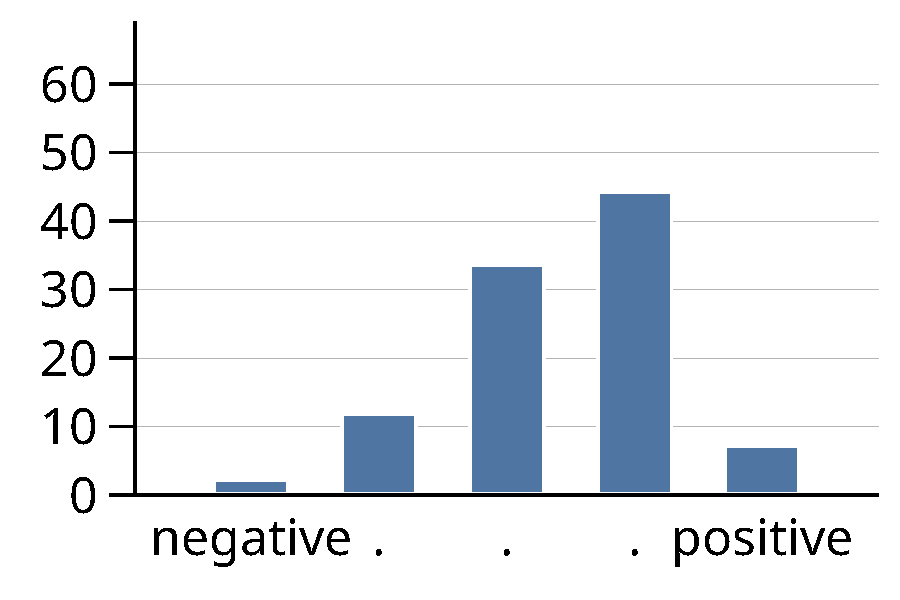
\includegraphics[width=1\linewidth]{descriptives/fig_ment_mh2.pdf}
    \caption{\code{mh2}: Well-balanced in the last 4 weeks}
    \label{fig:mh2}
\end{subfigure}\hfill%
  \begin{subfigure}{.30\textwidth}
    \includegraphics[width=1\linewidth]{descriptives/fig_ment_vt.pdf}
    \caption{\code{vt}: Physical pain in the last 4 weeks}
    \label{fig:vt}
\end{subfigure}\hfill%
  \\  %%%%%%%%%%%%%%%%%%%%%%%%%%%%%%%%%%%%%%%%%%%%%%%%%%%%%%%%%%%%%% newline 
  \begin{subfigure}{.30\textwidth}
    \includegraphics[width=1\linewidth]{descriptives/fig_ment_re1.pdf}
    \caption{\code{re1}: Accomplished less due to emotional problems}
    \label{fig:re1}
\end{subfigure}\hfill%
  \begin{subfigure}{.30\textwidth}
    \includegraphics[width=1\linewidth]{descriptives/fig_ment_re2.pdf}
    \caption{\code{re2}: Less careful due to emotional problems}
    \label{fig:re2}
\end{subfigure}\hfill%
  \begin{subfigure}{.30\textwidth}
    \includegraphics[width=1\linewidth]{descriptives/fig_ment_sf.pdf}
    \caption{\code{sf}: Limited socially due to health \phantom{text}}
    \label{fig:sf}
\end{subfigure}\hfill%
    \caption[Histogram of health variables used in the factor model]
    {Histogram of physical and mental health variables used in the factor model} \par \footnotesize
    \vspace{5pt} 
    Notes: Graphs depict proportion of categories so that they sum up to 100. 
    Labels recoded to order from `negative' to `positive' in terms of health outcome, independently of specific wording.
    For a detailed description on question wording, framing and recoding, see Table~\ref{tab:health_fact_varname_and_questions}.
    \label{fig:main_multifig_phys}
\end{figure}


